\documentclass[aspectratio=169]{beamer}
\usetheme{TUDelft}

% ====================================================================
% ANIMATION TOGGLE
% ====================================================================
\newif\ifanimated
\animatedtrue
\ifdefined\staticmode
  \animatedfalse
\fi
\newcommand{\cpause}{\ifanimated\pause\fi}

\usepackage{amsmath}
\usepackage{amssymb}
\usepackage{booktabs}
\usepackage{tikz}

% Import theme macros (includes TikZ libraries and semantic colors)
\usepackage{tikz}
\usetikzlibrary{positioning, shapes, arrows, shadows, fit, calc, decorations.pathreplacing}

% Semantic Colors - One meaning per color
\definecolor{irSparse}{HTML}{3498DB}   % Sparse/BM25: Blue
\definecolor{irDense}{HTML}{E67E22}    % Dense/Embeddings: Orange
\definecolor{irRerank}{HTML}{C0392B}   % Rerank/Cross-encoder: Red
\definecolor{irHybrid}{HTML}{2ECC71}   % Hybrid/Fusion: Green
\definecolor{irANN}{HTML}{9B59B6}      % ANN/Infra: Purple
\definecolor{irInfra}{HTML}{58595B}    % General Infra: Dark Gray
\definecolor{irMuted}{HTML}{D9D9D9}    % Faint Gray

% Base Styles - Consistent Diagram Grammar
\tikzset{
    irBoxBase/.style={
        rectangle, 
        draw, 
        rounded corners=2pt, 
        minimum height=0.8cm, 
        minimum width=2cm,
        font=\small\sffamily,
        align=center,
        drop shadow={opacity=0.15},
        inner sep=5pt
    },
    irDatabase/.style={
        cylinder, 
        draw, 
        shape border rotate=90, 
        aspect=0.25, 
        minimum height=1.2cm, 
        minimum width=1cm,
        fill=irMuted!20,
        draw=irInfra,
        font=\tiny\sffamily,
        align=center
    },
    % Semantic Variants
    sparse/.style={irBoxBase, fill=irSparse!10, draw=irSparse},
    dense/.style={irBoxBase, fill=irDense!10, draw=irDense},
    rerank/.style={irBoxBase, fill=irRerank!10, draw=irRerank},
    hybrid/.style={irBoxBase, fill=irHybrid!10, draw=irHybrid},
    ann/.style={irBoxBase, fill=irANN!10, draw=irANN},
    infra/.style={irBoxBase, fill=irInfra!10, draw=irInfra},
    % Legacy support / Utility
    muted/.style={irBoxBase, fill=irMuted!20, draw=irMuted!80!black, text=irMuted!50!black},
    ghost/.style={irBoxBase, fill=white, draw=irMuted!50, text=irMuted, dashed, drop shadow={opacity=0}},
    emph/.style={draw=irRerank, thick, drop shadow={shadow xshift=0mm, shadow yshift=0mm, fill=irRerank, opacity=0.3}},
    % Arrows
    irArrowBase/.style={->, thick, >=latex, draw=irInfra},
    irLabel/.style={
        font=\tiny\itshape, 
        text=irInfra, 
        align=center, 
        text width=2.5cm, 
        inner sep=3pt
    }
}


% =========================================================
% Stage Badge System
% =========================================================
% \irStage{StageName}
\newcommand{\irStage}[1]{%
    \begin{tikzpicture}[remember picture, overlay]
        \node[
            anchor=north east,
            fill=irInfra!10,
            text=irInfra,
            font=\tiny\bfseries,
            inner sep=3pt,
            rounded corners=1pt,
            yshift=-0.5cm,
            xshift=-0.5cm
        ] at (current page.north east) {#1};
    \end{tikzpicture}%
}

% =========================================================
% Math Highlighting
% =========================================================
% \mathhl[color]{content}
\newcommand{\mathhl}[2][irDense!30]{%
    \colorbox{#1}{$\displaystyle #2$}%
}

% =========================================================
% Math Vectors
% =========================================================
\newcommand{\vs}{\mathbf{s}}

% =========================================================
% Core Box Primitives
% =========================================================
% \IRBox[width]{id}{at}{title}{subtitle}{variant}
% Default width chosen for lecture slides; override when needed.
% \IRBox[width]{id}{at}{title}{subtitle}{variant}[extra options]
\DeclareDocumentCommand{\IRBox}{O{3.5cm} m m m m m O{}}{%
    \node[#6, text width=#1, #7] (#2) at #3 {%
        \textbf{#4}%
        \if\relax\detokenize{#5}\relax
        \else\\[-1mm]\scriptsize #5%
        \fi
    };%
}

% \IRWideBox{id}{at}{width}{title}{subtitle}{variant}
\newcommand{\IRWideBox}[6]{%
    \node[#6, text width=#3] (#1) at #2 {%
        \textbf{#4}%
        \if\relax\detokenize{#5}\relax
        \else\\[-1mm]\scriptsize #5%
        \fi
    };%
}

% =========================================================
% Arrow Primitives
% =========================================================
% Safe default: left-to-right flow
% \IRArrow{from}{to}{label}
\newcommand{\IRArrow}[3]{%
    \draw[irArrowBase] (#1.east) -- node[irArrowLabelAbove] {#3} (#2.west);%
}

% Explicit left-to-right
% \IRArrowLR{from}{to}{label}
\newcommand{\IRArrowLR}[3]{%
    \draw[irArrowBase] (#1.east) -- node[irArrowLabelAbove] {#3} (#2.west);%
}

% Explicit top-to-bottom
% \IRArrowTB{from}{to}{label}
\newcommand{\IRArrowTB}[3]{%
    \draw[irArrowBase] (#1.south) -- node[irArrowLabelRight] {#3} (#2.north);%
}

% Fully explicit anchor-to-anchor path
% \IRArrowPath{from anchor}{to anchor}{label}
% Example: \IRArrowPath{a.east}{b.north}{score}
\newcommand{\IRArrowPath}[3]{%
    \draw[irArrowBase] (#1) -- node[irArrowLabelAbove] {#3} (#2);%
}

% Orthogonal elbow path
% \IRArrowElbow{from anchor}{to anchor}{label}
% Example: \IRArrowElbow{a.east}{b.north}{feedback}
\newcommand{\IRArrowElbow}[3]{%
    \draw[irArrowBase] (#1) -| node[irArrowLabelBox] {#3} (#2);%
}

% Slanted arrow for special cases only
% \IRArrowSlanted{from anchor}{to anchor}{label}{pos}{width}
\newcommand{\IRArrowSlanted}[5]{%
    \draw[irArrowBase] (#1) -- node[above, sloped, irLabel, pos=#4, text width=#5, fill=white, inner sep=1pt] {#3} (#2);%
}

% =========================================================
% Accent Elements
% =========================================================
% \IRBadge{at}{text}
\newcommand{\IRBadge}[2]{%
    \node[
        draw=irAccent,
        fill=irAccent!20,
        rounded corners=1pt,
        font=\tiny\bfseries,
        inner sep=2pt
    ] at #1 {#2};%
}

% =========================================================
% Grouping
% =========================================================
% \IRGroup{fit nodes}{label}{variant}
% Example: \IRGroup{(a)(b)(c)}{First-stage retrieval}{muted}
\newcommand{\IRGroup}[3]{%
    \node[
        irGroupBase,
        #3,
        fit=#1
    ] (group) {};
    \node[
        anchor=north west,
        font=\tiny\bfseries,
        #3
    ] at ([xshift=2pt,yshift=-2pt] group.north west) {#2};%
}

% =========================================================
% Domain-Specific Shapes
% =========================================================
% \IRDocStack{id}{at}{label}
\newcommand{\IRDocStack}[3]{%
    \node[irDocStack] (#1) at #2 {#3};%
}

% \IRDatabase{id}{at}{label}
\newcommand{\IRDatabase}[3]{%
    \node[irDatabase] (#1) at #2 {#3};%
}

% =========================================================
% Layout Helpers
% =========================================================
% \IRPipelineTier{id}{at}{text}{label}{variant}
\newcommand{\IRPipelineTier}[5]{%
    \IRBox{#1}{#2}{#3}{}{#5}[]
    \node[anchor=west, irLabel, xshift=0.5cm] at (#1.east) {#4};%
}

% \IRTelescopeTier{id}{at}{width}{text}{variant}
\newcommand{\IRTelescopeTier}[5]{%
    \node[
        irTelescopeBase,
        #5,
        minimum width=#3
    ] (#1) at #2 {#4};%
}

% \IRStep{id}{at}{title}{subtitle}{variant}
% Creates a numbered step badge left of a box.
\newcommand{\IRStep}[5]{%
    \node[
        circle,
        draw=irAccent,
        fill=irAccent!20,
        font=\tiny\bfseries,
        inner sep=2pt
    ] (#1_num) at #2 {#1};
    \node[
        #5,
        text width=3.5cm,
        right=1.5cm of #1_num
    ] (#1) {%
        \textbf{#3}%
        \if\relax\detokenize{#4}\relax
        \else\\[-1mm]\scriptsize #4%
        \fi
    };
    \draw[irArrowBase, thin] (#1_num.east) -- (#1.west);%
}


\title{Learning to Rank}
\author{Avishek Anand}
\date{}

\begin{document}

% =====================================================
\begin{frame}[plain]
\titlepage
\end{frame}
% =====================================================

\begin{frame}{Overview}
\begin{itemize}
    \item What is ranking?
    \item Why is LTR hard?
    \item Pointwise methods
    \item Pairwise methods
    \item Listwise methods
    \item Metric-based methods
    \item Stochastic approaches
\end{itemize}
\end{frame}

% =====================================================
\section{The Ranking Problem}
% =====================================================

\begin{frame}{The Ranking Pipeline}
\begin{center}

\begin{tikzpicture}[node distance=2cm]
\node (query) [draw, rounded corners] {Query $q$};
\node (retrieve) [draw, right of=query, rounded corners] {Retrieve Candidates};
\node (features) [draw, right of=retrieve, rounded corners] {Feature Extraction};
\node (rank) [draw, right of=features, rounded corners] {Ranking Model};
\node (output) [draw, right of=rank, rounded corners] {Ranked List};

\draw[->] (query) -- (retrieve);
\draw[->] (retrieve) -- (features);
\draw[->] (features) -- (rank);
\draw[->] (rank) -- (output);
\end{tikzpicture}
\end{center}
\end{frame}

% =====================================================
\section{Motivation: Relevance Is Not King}
% =====================================================

% -----------------------------------------------------
\begin{frame}{Scenario 1: Product Search (E-commerce)}
\begin{center}
\fbox{
\begin{minipage}[c][4.3cm][c]{0.92\linewidth}
\centering
\Large
Screenshot Placeholder\\
(Product Search Results Page)
\end{minipage}
}
\end{center}

\vspace{0.6em}

\begin{columns}[T,onlytextwidth]
\column{0.34\textwidth}
\textbf{Objectives}
\begin{itemize}
  \item Relevance
  \item Revenue / margin
  \item Customer satisfaction
  \item Sponsored constraints
\end{itemize}

\column{0.33\textwidth}
\textbf{Features}
\begin{itemize}
  \item Text match (BM25/embeddings)
  \item Price + discounts
  \item Ratings / reviews
  \item Shipping speed, stock
  \item Seller quality
\end{itemize}

\column{0.33\textwidth}
\textbf{Feedback}
\begin{itemize}
  \item Clicks, add-to-cart
  \item Purchases/returns
  \item Position bias
  \item Promo effects
\end{itemize}
\end{columns}

\vspace{0.3em}
\centering
\alert{\large Relevance is not king.}
\end{frame}

% -----------------------------------------------------
\begin{frame}{Scenario 2: Academic Search (Scholar)}
\begin{center}
\fbox{
\begin{minipage}[c][4.3cm][c]{0.92\linewidth}
\centering
\Large
Screenshot Placeholder\\
(Google Scholar Results Page)
\end{minipage}
}
\end{center}

\vspace{0.6em}

\begin{columns}[T,onlytextwidth]
\column{0.34\textwidth}
\textbf{Objectives}
\begin{itemize}
  \item Relevance
  \item Authority / impact
  \item Recency (sometimes)
  \item Diversity of viewpoints
\end{itemize}

\column{0.33\textwidth}
\textbf{Features}
\begin{itemize}
  \item Text similarity
  \item Citations, PageRank-like
  \item Venue / author signals
  \item Year, topicality
\end{itemize}

\column{0.33\textwidth}
\textbf{Feedback}
\begin{itemize}
  \item Clicks / saves
  \item Citations (delayed)
  \item Popularity bias
  \item Interface position bias
\end{itemize}
\end{columns}

\vspace{0.3em}
\centering
\alert{\large Relevance is not king.}
\end{frame}

% -----------------------------------------------------
\begin{frame}{Scenario 3: Streaming (Netflix / Spotify)}
\begin{center}
\fbox{
\begin{minipage}[c][4.3cm][c]{0.92\linewidth}
\centering
\Large
Screenshot Placeholder\\
(Streaming Home Screen)
\end{minipage}
}
\end{center}

\vspace{0.6em}

\begin{columns}[T,onlytextwidth]
\column{0.34\textwidth}
\textbf{Objectives}
\begin{itemize}
  \item Engagement (watch time)
  \item Retention (long-term)
  \item Novelty / diversity
  \item Platform strategy
\end{itemize}

\column{0.33\textwidth}
\textbf{Features}
\begin{itemize}
  \item User/item embeddings
  \item Recent interactions
  \item Context (time/device)
  \item Similar-user patterns
\end{itemize}

\column{0.33\textwidth}
\textbf{Feedback}
\begin{itemize}
  \item Plays, skips
  \item Watch completion
  \item Dwell time is noisy
  \item Exposure bias
\end{itemize}
\end{columns}

\vspace{0.3em}
\centering
\alert{\large Relevance is not king.}
\end{frame}

% -----------------------------------------------------
\begin{frame}{Scenario 4: Online Advertising}
\begin{center}
\fbox{
\begin{minipage}[c][4.3cm][c]{0.92\linewidth}
\centering
\Large
Screenshot Placeholder\\
(Search Page with Ads)
\end{minipage}
}
\end{center}

\vspace{0.6em}

\begin{columns}[T,onlytextwidth]
\column{0.34\textwidth}
\textbf{Objectives}
\begin{itemize}
  \item Revenue
  \item User experience
  \item Advertiser value
  \item Policy / fairness constraints
\end{itemize}

\column{0.33\textwidth}
\textbf{Features}
\begin{itemize}
  \item Bid, predicted CTR
  \item Ad quality score
  \item Query-ad relevance
  \item User/context signals
\end{itemize}

\column{0.33\textwidth}
\textbf{Feedback}
\begin{itemize}
  \item Clicks, conversions
  \item Attribution noise
  \item Strategic bidding
  \item Strong position bias
\end{itemize}
\end{columns}

\vspace{0.3em}
\centering
\alert{\large Relevance is not king.}
\end{frame}

% =====================================================
% COMMONALITY SLIDE
% =====================================================

\begin{frame}{What Is Common Across All These Use Cases?}

\centering
\Large
We keep seeing the same pattern.

\bigskip
\pause

\begin{columns}[T,onlytextwidth]
\column{0.33\textwidth}
\textbf{Large feature space}
\begin{itemize}
  \item 100s--1000s signals
  \item strong interactions
\end{itemize}

\column{0.33\textwidth}
\textbf{Multi-objective}
\begin{itemize}
  \item relevance + business
  \item long-term vs short-term
\end{itemize}

\column{0.34\textwidth}
\textbf{Noisy feedback}
\begin{itemize}
  \item clicks are biased
  \item delayed outcomes
\end{itemize}
\end{columns}

\bigskip
\pause
\centering
\alert{\Large So how do we learn a good ranking function?}
\end{frame}

% =====================================================
% NEED FOR LTR
% =====================================================

\begin{frame}{Relevance is Multi-faceted}
% \irStage{BACKGROUND}
\textbf{Industrial search engines must optimize for more than just "topical" relevance.}

\vspace{0.8em}
\begin{columns}
\begin{column}{0.45\textwidth}
\begin{itemize}
    \item \textbf{Textual}: BM25, semantic match.
    \item \textbf{Quality}: Ratings, reviews.
    \item \textbf{Business}: Price, Prime shipping, revenue per click.
\end{itemize}\cpause
\end{column}
\begin{column}{0.5\textwidth}
\begin{center}

\includegraphics[width=\textwidth]{figures/search_amazon.png}
\end{center}
\end{column}
\end{columns}
\end{frame}

\begin{frame}{The Scale of Industrial Ranking}
% \irStage{BACKGROUND}
\textbf{Modern search giants handle a massive explosion of signals.}

\vspace{0.8em}
\begin{itemize}
    \item \textbf{Scope}: Amazon, eBay, and Google use **1000+ features** per document.
    \item \textbf{The Wall}: No human can manually tune $1000$ weights $\mathbf{w}$ to optimize a metric like NDCG.
    \item \textbf{Heterogeneity}: Combining BM25 (float) with "Is Fresh" (binary) and "Price" (currency).
\end{itemize}\cpause

\vspace{1em}
\cpause
\begin{alertblock}{The LTR Necessity}
We need a principled, automated way to learn the optimal "recipe" for combining these signals.
\end{alertblock}
\end{frame}

\begin{frame}{A Document as a Feature Vector}
% \irStage{BACKGROUND}
\textbf{Learning to Rank represents each query-document pair as a vector $\mathbf{x}$.}

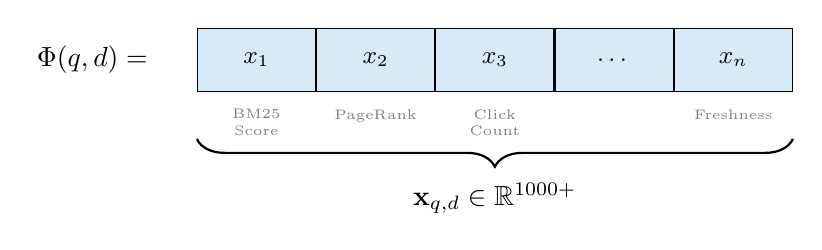
\begin{tikzpicture}[
    cell/.style={draw, minimum width=1.5cm, minimum height=0.8cm, font=\small},
    feat_label/.style={font=\tiny, gray, align=center}
]
\node[cell, fill=irSparse!20] (c1) {$x_1$};
\node[cell, fill=irSparse!20, right=0cm of c1] (c2) {$x_2$};
\node[cell, fill=irSparse!20, right=0cm of c2] (c3) {$x_3$};
\node[cell, fill=irSparse!20, right=0cm of c3] (c4) {$\dots$};
\node[cell, fill=irSparse!20, right=0cm of c4] (c5) {$x_n$};

\node[below=0.1cm of c1, feat_label] {BM25\\Score};
\node[below=0.1cm of c2, feat_label] {PageRank};
\node[below=0.1cm of c3, feat_label] {Click\\Count};
\node[below=0.1cm of c5, feat_label] {Freshness};

\node[left=0.5cm of c1, font=\normalsize] {$\Phi(q, d) = $};
\draw[decorate, decoration={brace, amplitude=10pt, mirror}, thick] ($(c1.south west)+(0,-0.6)$) -- ($(c5.south east)+(0,-0.6)$) node[midway, below=12pt] {$\mathbf{x}_{q,d} \in \mathbb{R}^{1000+}$};
\end{tikzpicture}

\vspace{1em}
\vspace{1em}
{\centering
\begin{tikzpicture}
    \IRBox{goal}{(0,0)}{The LTR Goal}{Learn $f(\mathbf{x}) \to \text{score}$ for optimal ranking}{hybrid}
\end{tikzpicture}
\par}


\end{frame}
%%%%%

\begin{frame}{Why Learning to Rank?}

\textbf{Problem:} We need a scoring function that combines many signals:
\[
s(q,d) = f(x_{q,d})
\]
where $x_{q,d}$ can have hundreds of components.

\bigskip

\begin{itemize}
  \item Hand-tuned rules do not scale (too many interactions).
  \item Objectives conflict (relevance vs revenue vs engagement).
  \item Supervision is weak and biased (implicit feedback).
\end{itemize}

\bigskip
\centering
\alert{\Large Learning to Rank is the engineering solution.}
\end{frame}

\begin{frame}{Where LTR Fits: The Multi-Stage Pipeline}
% \irStage{SYSTEM ARCHITECTURE}
\textbf{LTR is usually the final "re-ranking" stage in a complete stack.}

\vspace{0.5em}
\begin{center}
\resizebox{0.85\textwidth}{!}{
\begin{tikzpicture}[node distance=0.8cm]
    \IRBox[10cm]{s1}{(0,0)}{Stage 1: Sparse Retrieval (L3) \textit{or} Dense Retrieval (L5)}{}{sparse}[]
    \IRBox[10cm]{s1b}{(0,0)}{Optional: Query Expansion / PRF improves recall (L3)}{}{hybrid}[below=of s1]
    \IRBox[10cm]{s2}{(0,0)}{Stage 2: Neural Re-ranking / Cross-Encoder}{}{rerank}[below=of s1b]
    \IRBox[10cm]{s3}{(0,0)}{Stage 3: Learning to Rank (LTR) combines all signals (L6)}{Today}{hybrid}[below=of s2]
    \IRBox[10cm]{out}{(0,0)}{Final Ranked List $\to$ User or RAG Application}{}{infra}[below=of s3]

    \IRArrowTB{s1}{s1b}{}
    \IRArrowTB{s1b}{s2}{}
    \IRArrowTB{s2}{s3}{}
    \IRArrowTB{s3}{out}{}
\end{tikzpicture}

}
\end{center}

\cpause
\vspace{0.5em}
\begin{exampleblock}{The Funnel}
Sparse/Dense retrieval retrieves thousands; LTR perfectly orders the top 100.
\end{exampleblock}
\end{frame}

\begin{frame}{Recap: Why LTR is Necessary}
% \irStage{BACKGROUND}
\textbf{Our journey moved from hand-crafted matchers to complex neural-classical ensembles.}

\vspace{0.8em}
\begin{itemize}
    \item \textbf{L3--L4}: BM25 and BERT Cross-Encoders (Standard 2-stage pipeline).
    \item \textbf{L5}: Dense retrieval with Bi-Encoders and Late Interaction (ColBERT).
    \item \textbf{L5 (cont)}: Generative retrieval (DSI, SEAL).
\end{itemize}\cpause

\vspace{1em}
\cpause
\begin{block}{The Unasked Question}
How do we \textbf{train} these components together to optimize for the final ranking metrics we actually care about (NDCG, MAP)?
\end{block}
\end{frame}

\begin{frame}{Today's Goal: Directly Optimizing Rankings}
% \irStage{OBJECTIVE}
\textbf{The core problem is learning a scoring function that respects document ordering.}

\vspace{0.8em}
\begin{enumerate}
    \item \textbf{Pointwise}: Treat relevance as independent regression/classification.
    \item \textbf{Pairwise}: Learn relative preferences between pairs of documents.
    \item \textbf{Listwise}: Optimize the entire ranked permutation at once.
\end{enumerate}

\vspace{1em}
\cpause
\begin{block}{The Non-Differentiable Barrier}
Ranking metrics depend on \textbf{sorting}, which is discrete. We must find differentiable surrogates or smooth approximations to use Gradient Descent.
\end{block}
\end{frame}


\begin{frame}{The Learning to Rank Pipeline}
% \irStage{SYSTEM ARCHITECTURE}
\textbf{LTR separates feature extraction from the learned scoring and optimization logic.}

\vspace{0.8em}
\begin{itemize}
    \item \textbf{Traditional}: Hand-crafted features (BM25, PageRank) + LambdaMART.
    \item \textbf{Neural}: End-to-end representation learning + Ranking loss.
\end{itemize}\cpause

\vspace{0.5em}
\begin{center}
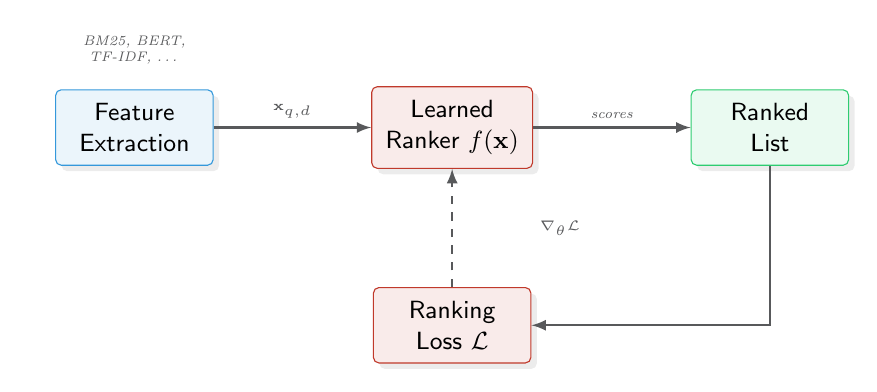
\begin{tikzpicture}[
    box/.style={irBoxBase, minimum height=1cm, minimum width=2.5cm},
    arr/.style={irArrowBase, thick}
]
\node[sparse] (feat) {Feature\\Extraction};
\node[rerank, right=2cm of feat] (model) {Learned\\Ranker $f(\mathbf{x})$};
\node[hybrid, right=2cm of model] (rank) {Ranked\\List};
\node[rerank, below=1.5cm of model] (loss) {Ranking\\Loss $\mathcal{L}$};

\draw[arr] (feat) -- node[above, irLabel, pos=0.5] {$\mathbf{x}_{q,d}$} (model);
\draw[arr] (model) -- node[above, irLabel, pos=0.5] {scores} (rank);
\draw[arr] (rank) |- (loss);
\draw[arr, dashed, irArrowBase] (loss) -- node[right, irLabel, pos=0.5] {$\nabla_\theta \mathcal{L}$} (model);

\node[above=0.2cm of feat, irLabel] {BM25, BERT, \\ TF-IDF, \ldots};
\end{tikzpicture}

\end{center}
\end{frame}

% =====================================================
\section{Evaluation Metrics --- What Are We Optimising?}
% =====================================================

\begin{frame}[plain]
\sectionpage
\end{frame}

\begin{frame}{Recap: Binary Metrics}
% \irStage{EVALUATION}
\textbf{Traditional metrics focus on whether a document is "relevant" or not.}

\vspace{0.8em}
\begin{itemize}
    \item \textbf{P@$k$ / R@$k$}: Good for broad recall but position-blind within top-$k$.
    \item \textbf{MRR}: Excellent for navigational/QA tasks (cares about first result).
    \item \textbf{MAP}: Averages precision across all relevant docs; sensitive to rank.
\end{itemize}\cpause

\vspace{1em}
\cpause
\begin{alertblock}{The Limitation}
Binary metrics ignore the \textbf{intensity} of relevance. In modern search, we often have graded labels (e.g., Perfect, Good, Fair, Bad).
\end{alertblock}
\end{frame}

\begin{frame}{NDCG: The Gold Standard for LTR}
% \irStage{EVALUATION}
\textbf{NDCG handles graded relevance and prioritizes top-heavy rankings.}

\vspace{0.8em}
\begin{itemize}
    \item \textbf{Grades}: Cumulative Gain (CG) sums relevance scores: $\sum \text{rel}_i$.
    \item \textbf{Discount}: DCG applies a logarithmic decay: $\sum \frac{\text{rel}_i}{\log_2(i+1)}$.
    \item \textbf{Normalization}: NDCG scales DCG to $[0, 1]$ relative to the ideal sort.
\end{itemize}\cpause

\vspace{0.5em}
\cpause
\begin{center}
\mathhl{\text{NDCG@}k = \frac{\sum_{i=1}^{k} \frac{2^{\text{rel}_i}-1}{\log_2(i+1)}}{\text{IDCG@}k}}
\end{center}
\end{frame}

\begin{frame}{Worked Example: Computing NDCG@5}
% \irStage{EVALUATION}
\textbf{Let's calculate the cost of a "miss" in the top positions.}

\vspace{0.8em}
\begin{itemize}
    \item \textbf{Current}: Grades $[2, 3, 1, 0, 0] \to \text{DCG} \approx 4.39$.
    \item \textbf{Ideal}: Grades $[3, 2, 1, 0, 0] \to \text{DCG} \approx 4.76$.
    \item \textbf{Result}: $\text{NDCG} = 4.39 / 4.76 \approx \mathbf{0.92}$.
\end{itemize}\cpause

\vspace{1em}
\cpause
\begin{exampleblock}{The Logarithmic Effect}
Notice that moving the "3" from position 1 to 2 caused an 8\% drop in score. NDCG is extremely sensitive to errors at the very top.
\end{exampleblock}
\end{frame}

% =====================================================

\begin{frame}{The Main Challenge for LTR}

\textbf{The sorting function (or the rank of a document) is difficult to optimize directly.}

\vspace{0.8em}
Ranking metrics (NDCG, MAP, etc.) as functions of document scores are:
\begin{itemize}
    \item \textbf{Non-smooth}
    \item \textbf{Mostly flat}
    \item \textbf{Discontinuous}
\end{itemize}

\bigskip
\begin{exampleblock}{The Derivative Problem}
Small score changes $\Rightarrow$ no metric change.\\
Tiny score swap $\Rightarrow$ big metric jump.
\end{exampleblock}

\vspace{0.5em}
\textbf{Gradients of the true metric are unusable. Each family of LTR methods has its own approach to overcoming this problem.}
\end{frame}

% =====================================================

\begin{frame}{Categorizing LTR methods?}

Most existing work describes three categories: \textbf{Pointwise, Pairwise and Listwise}.

\vspace{0.8em}
\cpause
Despite wide usage:
\begin{itemize}
    \item There is not a clear consistently-used definition of each.
    \item Some methods are categorized differently by different works.
    \item It is not useful to see them as strictly non-overlapping categories.
\end{itemize}

\vspace{0.8em}
\cpause
\begin{alertblock}{A Better Perspective}
Think in terms of \textbf{properties} instead of categories.
\end{alertblock}
\end{frame}

% =====================================================
\section{Pointwise Approaches}
% =====================================================

\begin{frame}[plain]
\sectionpage
\end{frame}

\begin{frame}{1. Where Do Labels Come From?}
% \irStage{DATA}
\textbf{To train a model, we need target labels $y$ for query-document pairs.}

\vspace{0.8em}
\begin{itemize}
    \item \textbf{Explicit Ratings}: Human judges grade relevance (e.g., 0=Bad to 4=Perfect). Expensive but high quality.
    \item \textbf{Implicit Feedback}: User behavior parsed from logs.
    \begin{itemize}
        \item \textbf{Clicks}: Did the user click? (Binary)
        \item \textbf{Dwell Time}: How long did they stay?
        \item \textbf{Skips}: Did they scroll past it?
    \end{itemize}
\end{itemize}
\end{frame}

\begin{frame}{2. The Training Table}
% \irStage{DATA}
\textbf{We flatten the data into a standard machine learning dataset.}

\vspace{0.8em}
Each row is an isolated instance: a Query $q$, a Document $d$, their extracted features $\mathbf{x}$, and the target label $y$.

\vspace{1em}
\begin{center}
\small
\begin{tabular}{cc | ccc | c}
\toprule
\textbf{Query ID} & \textbf{Doc ID} & \textbf{BM25 ($x_1$)} & \textbf{PageRank ($x_2$)} & \dots & \textbf{Label ($y$)} \\
\midrule
$q_1$ & $d_A$ & 12.4 & 0.85 & \dots & \textcolor{green!70!black}{\textbf{1 (Click)}} \\
$q_1$ & $d_B$ & 8.1 & 0.92 & \dots & \textcolor{red}{\textbf{0 (Skip)}} \\
$q_1$ & $d_C$ & 15.2 & 0.12 & \dots & \textcolor{green!70!black}{\textbf{1 (Click)}} \\
\midrule
$q_2$ & $d_X$ & 5.5 & 0.44 & \dots & \textcolor{red}{\textbf{0 (Skip)}} \\
\bottomrule
\end{tabular}
\end{center}
\vspace{0.5em}
\begin{exampleblock}{Key Insight}
The model sees rows independently. It does not know that $d_A, d_B, d_C$ belong to the same query $q_1$ during the forward pass.
\end{exampleblock}
\end{frame}

\begin{frame}{3. Mapping Features to a Score}
% \irStage{MODELS}
\textbf{A Pointwise model $f(\mathbf{x})$ maps the feature vector to a predicted score $\hat{y}$.}

\vspace{0.8em}
\begin{itemize}
    \item \textbf{Linear Model}: $\hat{y} = \mathbf{w}^\top \mathbf{x} + b$. (Fast, but assumes linear relationships).
    \item \textbf{Neural Network}: $\hat{y} = \text{MLP}(\mathbf{x})$. (Captures complex feature interactions).
    \item \textbf{Tree Ensemble}: $\hat{y} = \sum \text{Tree}(\mathbf{x})$. (Handles heterogeneous features well).
\end{itemize}
\end{frame}

\begin{frame}{4. The Pointwise Loss per Example}
% \irStage{MODELS}
\textbf{We train the model to minimize the error between prediction $\hat{y}$ and label $y$.}

\vspace{0.8em}
\begin{itemize}
    \item \textbf{Regression} (e.g., MSE): $\mathcal{L} = (y - \hat{y})^2$
    \item \textbf{Classification} (e.g., BCE): $\mathcal{L} = -y \log(\hat{y}) - (1-y)\log(1-\hat{y})$
\end{itemize}

\vspace{1em}
\cpause
\begin{block}{What is it actually doing?}
For $q_1, d_A$, the loss penalizes the model if $\hat{y}$ is far from $1$. It updates the weights $\theta$ to make $\hat{y}$ closer to $1$ \textbf{in isolation}.
\end{block}
\end{frame}

% =====================================================

\begin{frame}{Limitation of Pointwise Methods}
\textbf{Pointwise losses do not directly optimize ranking quality. A lower loss does not mean a better ranking!}

\vspace{0.8em}
\begin{columns}[T]
\begin{column}{0.48\textwidth}
\begin{block}{Model A}
\centering
\begin{tabular}{ccc}
\toprule
\textbf{Rel.} & \textbf{Score} & \textbf{Rank} \\
\midrule
1 & 0.6 & 1 \\
0 & 0.5 & 2 \\
0 & 0.5 & 3 \\
0 & 0.5 & 4 \\
0 & 0.5 & 5 \\
\bottomrule
\end{tabular}
\end{block}
\end{column}

\begin{column}{0.48\textwidth}
\begin{alertblock}{Model B}
\centering
\begin{tabular}{ccc}
\toprule
\textbf{Rel.} & \textbf{Score} & \textbf{Rank} \\
\midrule
1 & 0.1 & 5 \\
0 & 0.2 & 1 \\
0 & 0.2 & 2 \\
0 & 0.2 & 3 \\
0 & 0.2 & 4 \\
\bottomrule
\end{tabular}
\end{alertblock}
\end{column}
\end{columns}

\vspace{1em}
\textbf{Mismatch}: Ranking is fundamentally about the \textbf{relative order} of documents, not fitting a curve.
\end{frame}

\begin{frame}{Pointwise in Disguise: Standard Cross-Encoders}
% \irStage{RE-RANKING}
\textbf{Recall monoBERT from Lecture 4 is technically a pointwise ranker.}

\vspace{0.8em}
\begin{itemize}
    \item \textbf{Input}: Joint query-document sequence \texttt{[CLS] Q [SEP] D}.
    \item \textbf{Loss}: Binary Cross-Entropy on the \texttt{[CLS]} representation.
    \item \textbf{Success}: Works well because BERT captures deep semantics, but \textbf{not} because the loss is optimal for ranking.
\end{itemize}\cpause

\vspace{1em}
\cpause
\begin{exampleblock}{The Capacity Paradox}
With enough data and model capacity (like LLMs), simplistic pointwise losses often reach surprisingly high performance.
\end{exampleblock}
\end{frame}

% =====================================================
\section{Pairwise Approaches}
% =====================================================

\begin{frame}[plain]
\sectionpage
\end{frame}

\begin{frame}{Pairwise: Relative Preferences}
% \irStage{PARADIGMS}
\textbf{Instead of absolute scores, we learn which document is "better" in a pair.}

\vspace{0.8em}
\begin{itemize}
    \item \textbf{Intuition}: For each pair $(d_i, d_j)$, if $y_i > y_j$, the model should score $s_i > s_j$.
    \item \textbf{Strength}: Transforms ranking into binary classification of pairs.
    \item \textbf{Feedback}: Errors are symmetric --- push one up, the other down.
\end{itemize}\cpause

\vspace{0.5em}
\begin{center}
\begin{tikzpicture}[
    doc/.style={irBoxBase, minimum height=0.7cm, minimum width=1.5cm},
    arr/.style={irArrowBase, thick}
]
\node[hybrid] (d1) {$d_i$\\ \tiny (rel=3)};
\node[rerank, right=3cm of d1] (d2) {$d_j$\\ \tiny (rel=1)};
\node[below=1.2cm of $(d1)!0.5!(d2)$, info] (pred) {$f(\mathbf{x}_i) > f(\mathbf{x}_j)$ ?};

\draw[arr, irHybrid] (d1) -- node[above, irLabel, pos=0.5] {should rank higher} (d2);
\draw[arr, dashed, irInfra] (d1) |- (pred);
\draw[arr, dashed, irInfra] (d2) |- (pred);

\node[below=0.1cm of pred, irLabel, text width=4cm] {Goal: Maximize agreement with labels};
\end{tikzpicture}

\end{center}
\end{frame}

\begin{frame}{RankNet: Learning from Pairs}
% \irStage{MODELS}
\textbf{Pairwise loss minimizes the average number of pair-inversions in rankings.}

\vspace{0.8em}
For all pairs where $y_i > y_j$:
\[
\mathcal{L}_{pair} = \sum_{y_i > y_j} \phi(s_i - s_j)
\]

\vspace{0.8em}
\textbf{RankNet} is the most prominent pairwise method:
\[
\mathcal{L}_{RankNet} = \sum_{y_i > y_j} \log(1 + e^{-(s_i - s_j)})
\]

\vfill
\footnotesize \textit{Burges, C. et al. Learning to rank using gradient descent. ICML 2005.}
\end{frame}

% =====================================================

\begin{frame}{Limitation of Pairwise Methods}
\textbf{We minimize incorrect inversions. However, not every pair is equally important.}

\vspace{0.8em}
\begin{columns}[T]
\begin{column}{0.48\textwidth}
\begin{block}{Ranking 1}
\centering
\begin{tabular}{ccc}
\toprule
\textbf{Rel.} & \textbf{Score} & \textbf{Rank}\\
\midrule
1 & 0.6 & 1\\
0 & 0.2 & 4\\
1 & 0.1 & 5\\
0 & 0.4 & 3\\
0 & 0.8 & 2\\
\bottomrule
\end{tabular}\\
\vspace{0.3em}
\textbf{Pairs correct: 9}
\end{block}
\end{column}

\begin{column}{0.48\textwidth}
\begin{alertblock}{Ranking 2}
\centering
\begin{tabular}{ccc}
\toprule
\textbf{Rel.} & \textbf{Score} & \textbf{Rank}\\
\midrule
0 & 0.8 & 1\\
0 & 0.6 & 2\\
1 & 0.4 & 3\\
0 & 0.2 & 4\\
1 & 0.1 & 5\\
\bottomrule
\end{tabular}\\
\vspace{0.3em}
\textbf{Pairs correct: 10}
\end{alertblock}
\end{column}
\end{columns}

\vspace{1em}
\textbf{Mismatch}: It's much more important to get the correct ordering of top documents than bottom ones. Pairwise treats all pairs equally.
\end{frame}

\begin{frame}{Worked Example: RankNet Misstep}
% \irStage{MODELS}
\textbf{Suppose a Blog (rel=1) is scored at 2.5, while a Tier-1 list (rel=3) is at 2.1.}

\vspace{0.8em}
\begin{itemize}
    \item \textbf{Conflict}: $P(\text{Tier-1} \succ \text{Blog}) \approx 0.40$ (Model is wrong).
    \item \textbf{Gradient}: Pushes Tier-1 score up ($+0.60$) and Blog down ($-0.60$).
    \item \textbf{Observation}: RankNet weights all swaps equally, regardless of position.
\end{itemize}\cpause

\vspace{1em}
\cpause
\begin{alertblock}{The Position Blindness}
Swapping docs at positions 1--2 should be "more important" than positions 99--100. RankNet's loss doesn't know about positions.
\end{alertblock}
\end{frame}

\begin{frame}{RankSVM: Margin-Based Ranking}
% \irStage{MODELS}
\textbf{Historical significance: First to use implicit feedback (clicks) for LTR.}

\vspace{0.8em}
\begin{itemize}
    \item \textbf{Margin}: Force $\mathbf{w}^\top (\mathbf{x}_i - \mathbf{x}_j) \geq 1$ for correctly ordered pairs.
    \item \textbf{Feed}: Users clicking result $i$ after skipping $j \implies d_i \succ d_j$.
    \item \textbf{Legacy}: Solid theory (max-margin) but less scalable than boosting.
\end{itemize}\cpause

\vspace{1em}
\cpause
\begin{exampleblock}{Key Contribution}
Joachims (2002) showed that even noisy implicit signals (clicks) can train a competitive ranker when framed as a pairwise problem.
\end{exampleblock}
\end{frame}

% =====================================================
\section{Listwise Approaches}
% =====================================================

\begin{frame}[plain]
\sectionpage
\end{frame}

\begin{frame}{Listwise: Optimising the Distribution}
% \irStage{PARADIGMS}
\textbf{Listwise models treat the entire set of documents as a single unit.}

\vspace{0.8em}
\begin{itemize}
    \item \textbf{Philosophy}: Don't look at doc pairs; look at the \textit{permutation}.
    \item \textbf{Models}: $P(\text{ranking} \mid \text{scores})$ is modelled as a probability distribution.
    \item \textbf{Loss}: Minimize KL-divergence between predicted and ideal distributions.
\end{itemize}\cpause

\vspace{0.5em}
\begin{center}
\begin{tikzpicture}[
    box/.style={irBoxBase, minimum height=0.7cm, minimum width=2cm},
    arr/.style={irArrowBase, thick}
]
\node[listwise] (perm) {Permutation\\$\pi \in \mathcal{S}_n$};
\node[rerank, right=2cm of perm] (loss) {Listwise Loss\\$P(\pi_y \mid \vs)$};
\node[below=1.2cm of $(perm)!0.5!(loss)$, info] (prob) {Score all docs jointly};

\draw[arr, irListwise] (perm) -- node[above, irLabel] {calculate} (loss);
\draw[arr, dashed, irInfra] (prob) -- (perm);
\draw[arr, dashed, irInfra] (prob) -- (loss);

\node[below=0.1cm of prob, irLabel, text width=5cm] {Goal: Minimize distance between predicted and ideal permutations};
\end{tikzpicture}

\end{center}
\end{frame}

\begin{frame}{Connection: Knowledge Distillation as LTR}
% \irStage{RE-RANKING}
\textbf{Teaching a Bi-Encoder (Student) to mimic a Cross-Encoder (Teacher) is a ranking task.}

\vspace{0.8em}
\begin{itemize}
    \item \textbf{Teacher}: Provides graded relevance scores for top-$k$ documents.
    \item \textbf{Student}: Must learn to reproduce the relative ordering, not just absolute scores.
    \item \textbf{Losses}: Listwise KL-divergence over softmaxes works best.
\end{itemize}\cpause

\vspace{1em}
\cpause
\begin{exampleblock}{TAS-B Result}
Using pairwise/listwise distillation significantly outperforms simple MSE on the MS MARCO benchmark.
\end{exampleblock}
\end{frame}

\begin{frame}{Listwise LTR Methods (Plackett-Luce)}

\textbf{Listwise methods consider the entire ranking in their loss.}

\vspace{0.8em}
The first listwise method (ListNet) optimizes a Soft-Max \textbf{Plackett-Luce} distribution.
Ranking is formulated as sequential sampling without replacement:

\[
P(\pi | s) = \prod_{k=1}^{n} \frac{e^{s_{\pi_k}}}{\sum_{j=k}^{n} e^{s_{\pi_j}}}
\]

\vspace{0.8em}
Loss minimizes the cross-entropy with the "best possible" ranking.

\vfill
\footnotesize \textit{Cao, Z. et al. Learning to rank: from pairwise... to listwise approach. ICML 2007.}
\end{frame}

% =====================================================

\begin{frame}{Limitation of Early Listwise Methods}

\textbf{ListNet assumes there is a single best ranking and optimizes its likelihood.}

\vspace{0.8em}
\begin{alertblock}{The Metric Disconnect}
Likelihood maximization \textbf{does not directly optimize} NDCG or MAP.
\end{alertblock}

\vspace{0.8em}
Improved likelihood $\neq$ improved evaluation metric. 

There is no actual ranking metric involved in original Listwise methods.
\end{frame}

% =====================================================
\section{Metric-Based Methods \& LambdaMART}
% =====================================================

\begin{frame}[plain]
\sectionpage
\end{frame}

\begin{frame}{Metric-Based LTR Methods (LambdaRank)}
% \irStage{MODELS}
\textbf{Metric-based LTR aims to optimize a specific ranking metric directly.}

\vspace{0.8em}
Almost all ranking metrics are listwise, thus metric-based implies listwise.

The most-influential metric-based method is \textbf{LambdaRank}. It takes the Pairwise loss of RankNet, and weights each pair by how much swapping them affects the metric (e.g., $|\Delta \text{NDCG}|$):

\[
\mathcal{L}_{\text{LambdaRank}} = \sum_{y_i > y_j} \log(1 + e^{-(s_i - s_j)}) \cdot |\Delta \text{NDCG}|
\]

\vspace{0.8em}
The gradients treat these weights as constants. Focus is on errors at the top!

\vfill
\footnotesize \textit{Burges, C. J. et al. Learning to rank with nonsmooth cost functions. NIPS 2006.}
\end{frame}

\begin{frame}{The Lambda Insight}
% \irStage{THEORY}
\textbf{LambdaRank defines gradients directly, without an explicit loss function.}

\vspace{0.8em}
\begin{itemize}
    \item \textbf{Problem}: NDCG is non-differentiable (jumpy).
    \item \textbf{Solution}: Specify the physical "force" ($\lambda$) acting on each doc.
    \item \textbf{Analogy}: "Pull" relevant docs up, "push" irrelevant ones down.
\end{itemize}\cpause

\vspace{1em}
\cpause
\begin{alertblock}{A Theory Mystery}
Surprisingly, optimizing these gradients leads to a local optimum for the target ranking metric (Burges et al., 2006).
\end{alertblock}
\end{frame}

\begin{frame}{Worked Example: Lambda Power}
% \irStage{THEORY}
\textbf{Correcting errors at the top yields much higher "gravitational" force.}

\vspace{0.8em}
\begin{itemize}
    \item \textbf{Top Swap} (Pos 1--2): Resulting $|\Delta\text{NDCG}| = \mathbf{0.154}$.
    \item \textbf{Bottom Swap} (Pos 3--4): Resulting $|\Delta\text{NDCG}| = \mathbf{0.030}$.
    \item \textbf{Impact}: The top swap exerts 5$\times$ more gradient force on the model than the bottom swap.
\end{itemize}\cpause

\vspace{1em}
\cpause
\begin{exampleblock}{Convergence}
This weighting causes the model to "give up" on tail documents and focus exclusively on perfecting the top-10 results.
\end{exampleblock}
\end{frame}

\begin{frame}{LambdaMART: Industry Workhorse}
% \irStage{MODELS}
\textbf{Combines Lambda gradients with Gradient Boosted Regression Trees.}

\vspace{0.8em}
\begin{itemize}
    \item \textbf{MART}: Multiple Additive Regression Trees (Boosting).
    \item \textbf{Process}: Compute current $\lambda$ for all docs $\to$ Fit a tree to predict those $\lambda$ values $\to$ Add tree to ensemble.
    \item \textbf{Standard}: Powering Bing, Yahoo, and specialized e-commerce search for years.
\end{itemize}\cpause

\vspace{1em}
\cpause
\begin{exampleblock}{Why Trees?}
Non-neural trees handle \textbf{heterogeneous features} (BM25 score + PageRank + Category ID) much better than MLPs without massive feature engineering.
\end{exampleblock}
\end{frame}

\begin{frame}{LTR Features: What the Model "Sees"}
% \irStage{DATA}
\textbf{Traditional LTR models use a large bank of query-document features.}

\vspace{0.8em}
\begin{itemize}
    \item \textbf{Lexical}: BM25, TF-IDF, Language Model scores.
    \item \textbf{Structural}: In-link count (PageRank), URL length, title matches.
    \item \textbf{Modern}: Dense similarity (L5), Cross-encoder scores (L4).
\end{itemize}\cpause

\vspace{1em}
\cpause
\begin{alertblock}{The Ensemble Effect}
LambdaMART doesn't replace BM25; it uses BM25 as \textbf{one of many inputs}. It learns the optimal "mixture" of classical and semantic signals.
\end{alertblock}
\end{frame}

% =====================================================

\begin{frame}{Rank Metric Approximation}

\textbf{ApproxDCG approximates the rank function through a sigmoid upper bound.}

\vspace{0.8em}
\[
\hat{\text{rank}}_i = 1 + \sum_{j \neq i} \sigma(s_j - s_i)
\]

\vspace{0.8em}
This differentiable approximate rank is then plugged into the DCG objective:
\[
\text{ApproxDCG} = \sum_{i=1}^n \frac{2^{y_i} - 1}{\log_2(1 + \hat{\text{rank}}_i)}
\]

\vfill
\footnotesize \textit{Qin, T. et al. A general approximation framework for direct optimization... IRJ 2010.}
\end{frame}

\begin{frame}{The Modern Retrieve-Then-Rerank Stack}
% \irStage{SYSTEM ARCHITECTURE}
\textbf{Modern search engines are multi-stage ensembles of different LTR paradigms.}

\vspace{0.8em}
\begin{itemize}
    \item \textbf{Stage 1}: Dense/Sparse Retrieval (Recall optimized, Pointwise InfoNCE).
    \item \textbf{Stage 2}: Neural Re-ranker (High interaction, Pairwise BERT).
    \item \textbf{Stage 3}: LambdaMART (Aggregates all signals + metadata).
\end{itemize}\cpause

\vspace{1em}
\cpause
\begin{center}
\begin{tikzpicture}[node distance=3cm]
    \IRBox{s1}{(0,0)}{Lexical}{Recall}{sparse}
    \IRBox{s2}{(4,0)}{Neural}{Precision}{dense}
    \IRBox{s3}{(8,0)}{Ensemble}{Ranking}{hybrid}
    \draw[irArrowBase] (s1) -- (s2);
    \draw[irArrowBase] (s2) -- (s3);
\end{tikzpicture}
\end{center}
\end{frame}

\begin{frame}[fragile]{Practical LTR: LightGBM \& PyTerrier}
% \irStage{HANDS-ON}
\textbf{Standardized libraries make it easy to train metric-aware rankers.}

\vspace{0.8em}
\begin{itemize}
    \item \textbf{LightGBM}: The primary engine for LambdaMART in industrial search.
    \item \textbf{PyTerrier}: Orchestrates the pipeline from indexing to ensemble training.
    \item \textbf{Objective}: Simply set \texttt{"objective": "lambdarank"} to start.
\end{itemize}\cpause

\vspace{0.5em}
\cpause
\begin{exampleblock}{Feature BANK}
The power of LambdaMART comes from its ability to use \textbf{50+ features}: BM25, PageRank, BERT scores, and URL statistics.
\end{exampleblock}
\end{frame}

% =====================================================
\section{Stochastic Methods}
% =====================================================

\begin{frame}{Stochastic LTR Methods}

\textbf{Inspired by reinforcement learning, optimize the expected utility of a probabilistic ranking model:}

\vspace{0.8em}
\[
\mathbb{E}_{R \sim \pi_\theta} [\text{Metric}(R)]
\]

The number of possible rankings is enormous, so it is only feasible to approximate this expected value via \textbf{sampling}.

\vspace{0.8em}
\textbf{The REINFORCE log-derivative trick} approximates the gradient from samples:
\[
\nabla_\theta \mathbb{E}_{R \sim \pi_\theta} [\text{Metric}(R)] = \mathbb{E}_{R \sim \pi_\theta} [\text{Metric}(R) \nabla_\theta \log P(R | \theta)]
\]

\vfill
\footnotesize \textit{Oosterhuis, H. Computationally efficient optimization of Plackett-Luce ranking... SIGIR 2021.}
\end{frame}

% =====================================================

% =====================================================

\begin{frame}{Big Picture Comparison}
\begin{tabular}{l l}
\toprule
Method & What It Optimizes \\
\midrule
Pointwise & Regression/classification loss \\
Pairwise & Pair inversions \\
Listwise & Ranking likelihood \\
Metric-based & Metric-informed gradients \\
Stochastic & Expected metric \\
\bottomrule
\end{tabular}
\end{frame}

% ====================================================================
\section{Beyond Standard LTR: Counterfactual \& Online}
% ====================================================================

\begin{frame}[plain]
\sectionpage
\end{frame}

\begin{frame}{The Problem with Clicks: Position Bias}
% \irStage{DATA}
\textbf{Implicit feedback (clicks) is cheap and abundant, but heavily biased.}

\vspace{0.8em}
\begin{itemize}
    \item \textbf{Position Bias}: Users are much more likely to click the top result simply because it is at the top, \textit{even if it's less relevant} than the result at position 3.
    \item \textbf{The Echo Chamber}: If we train LTR directly on raw clicks, the model learns to reproduce the existing biased ranking!
    \item \textbf{Trust Bias}: Users trust the search engine and might click a bad top result before realizing it's useless (hence, "skips" and "dwell time" help, but don't cure the bias).
\end{itemize}\cpause

\vspace{1em}
\cpause
\begin{alertblock}{The Counterfactual Question}
"Would the user have clicked Document B if it had been shown at Position 1 instead of Document A?"
\end{alertblock}
\end{frame}

\begin{frame}{Counterfactual LTR (CLTR): Inverse Propensity Scoring}
% \irStage{MODELS}
\textbf{CLTR attempts to un-bias the click data during training.}

\vspace{0.8em}
\begin{columns}
\begin{column}{0.5\textwidth}
\begin{itemize}
    \item \textbf{Propensity ($p_k$)}: The probability a user \textit{examines} position $k$. ($p_1 = 1.0, p_3 = 0.4$).
    \item \textbf{IPS Weighting}: Up-weight clicks that happen at lower, less-examined positions.
    \item \textbf{Example}: A click at position 3 ($p=0.4$) is worth $1/0.4 = \mathbf{2.5\times}$ more heavily in the loss than a click at position 1.
\end{itemize}
\end{column}
\begin{column}{0.45\textwidth}
\begin{center}
% PLACEHOLDER IMAGE
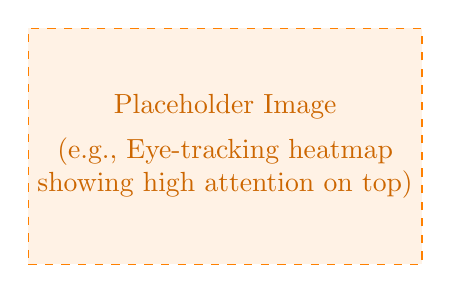
\begin{tikzpicture}
    \node[draw=orange, dashed, fill=orange!10, minimum width=4.5cm, minimum height=3cm, align=center, text=orange!80!black] {Placeholder Image\\[4pt](e.g., Eye-tracking heatmap\\showing high attention on top)};
\end{tikzpicture}
\end{center}
\end{column}
\end{columns}

\vspace{0.5em}
\cpause
\begin{exampleblock}{The Result}
By weighting by $1/p_k$, we create an unbiased estimator of true relevance from biased click logs.
\end{exampleblock}
\end{frame}

\begin{frame}{The Problem with Offline LTR: Static Datasets}
% \irStage{DATA}
\textbf{Training on historical Data ($X, Y$) assumes the world stands still.}

\vspace{0.8em}
\begin{itemize}
    \item \textbf{Concept Drift}: What is relevant for "apple" today (iPhone 15) is different from what was relevant 6 months ago (iPhone 14).
    \item \textbf{Cold Start}: New documents have no historical click data or explicit ratings.
    \item \textbf{Expensive Updates}: Re-training a massive LambdaMART ensemble and deploying it takes days or weeks.
\end{itemize}\cpause

\vspace{1em}
\cpause
\begin{alertblock}{The Static Limitation}
Standard LTR models degrade over time because they cannot adapt immediately to breaking news, viral trends, or shifting user intents.
\end{alertblock}
\end{frame}

\begin{frame}{Online LTR (OLTR): Learning from Live Interactions}
% \irStage{MODELS}
\textbf{OLTR models learn directly and immediately by interacting with users.}

\vspace{0.8em}
\begin{columns}
\begin{column}{0.5\textwidth}
\begin{itemize}
    \item \textbf{Exploration vs. Exploitation}: We must safely test new ranking strategies without ruining the user experience.
    \item \textbf{Interleaving}: Combine the results of Ranker A (current) and Ranker B (new) by alternating them.
    \item \textbf{Dueling Bandits (DBGD)}: Whichever ranker gets more clicks in the interleaved list "wins", and the model updates in that direction immediately.
\end{itemize}
\end{column}
\begin{column}{0.45\textwidth}
\begin{center}
% PLACEHOLDER IMAGE
\begin{tikzpicture}
    \node[draw=irListwise, dashed, fill=irListwise!10, minimum width=4.5cm, minimum height=3cm, align=center, text=irListwise!80!black] {Placeholder Image\\[4pt](e.g., Team Draft Interleaving\\Ranker A vs Ranker B)};
\end{tikzpicture}
\end{center}
\end{column}
\end{columns}
\end{frame}

% ====================================================================
\section{Summary: Choosing Your Paradigm}
% ====================================================================

\begin{frame}[plain]
\sectionpage
\end{frame}

\begin{frame}{Summary: Choosing Your Paradigm}
% \irStage{SUMMARY}
\textbf{The trade-off is between ranking awareness and computational complexity.}

\vspace{0.8em}
\begin{itemize}
    \item \textbf{Pointwise}: Fast, scalable, but position-blind. Best for 1st stage.
    \item \textbf{Pairwise}: The standard for re-ranking. LambdaMART is the workhorse.
    \item \textbf{Listwise}: Use for deep semantic interaction or small top-$k$ re-ranking.
\end{itemize}\cpause

\vspace{1em}
\cpause
\begin{alertblock}{The Recall Ceiling}
Remember: A perfect re-ranker cannot fix what the first stage missed. LTR is most effective when the retrieval stage has high recall.
\end{alertblock}
\end{frame}

\begin{frame}{Next Class: Evaluation \& Large Scale Systems}
% \irStage{SUMMARY}
\textbf{Next week, we move into the "wild" --- how to evaluate systems with real users.}

\vspace{0.8em}
\begin{itemize}
    \item \textbf{Offline}: Benchmarks like TREC and the limits of static labels.
    \item \textbf{Online}: A/B testing, Interleaving, and Click-through analysis.
    \item \textbf{Deployment}: Building low-latency production pipelines.
\end{itemize}\cpause

\vspace{1em}
\cpause
\begin{block}{Preparation}
Review the PyTerrier documentation for the Learning to Rank module.
\end{block}
\end{frame}

% =====================================================

\appendix
\end{document}